\subsection{An\'alisis tercera iteraci\'on de datos de sensores para implementaci\'on de aplicaci\'on m\'ovil} % (fold)
\label{sub:An\'alisis tercera }
    En esta tercera iteraci\'on, se realizaron pruebas en un entorno al aire libre con el objetivo de evaluar el 
        comportamiento del sistema bajo condiciones de luz natural intensa, especialmente luz solar directa. 
        Estas pruebas eran fundamentales para determinar c\'omo se desempe\~naba el sensor LiDAR en exteriores, 
        ya que la aplicaci\'on m\'ovil debe poder funcionar en entornos tanto interiores como exteriores.
    \vskip 0.5cm
    Durante las pruebas, se observ\'o que la luz del sol afectaba negativamente la capacidad del LiDAR para 
        detectar obst\'aculos. Este problema es causado por la emisi\'on de se\~nales infrarrojas por parte del 
        sol, que interfieren con las longitudes de onda que el LiDAR utiliza para medir distancias. Como 
        consecuencia, el sensor mostr\'o dificultades para identificar correctamente los obst\'aculos en \'areas 
        donde la luz solar incid\'ia directamente. En algunos casos, los objetos cercanos no eran detectados 
        o se detectaban de manera incorrecta, lo que compromete la capacidad del robot para evitar obst\'aculos 
        en entornos al aire libre bajo luz solar intensa.
    \vskip 0.5cm
    Adem\'as de esta interferencia causada por la luz solar, se identific\'o otro problema en el comportamiento del 
        LiDAR cuando los objetos se encontraban a menos de 10 cm del sensor. A estas distancias tan cortas, 
        el LiDAR detecta los objetos como si estuvieran extremadamente cerca, lo que distorsiona la 
        representaci\'on en el minimapa y provoca errores en la visualizaci\'on de los obst\'aculos. Sin embargo, 
        a pesar de que el mapeo no es preciso en estas condiciones, el sistema sigue siendo capaz de esquivar 
        los obst\'aculos en la mayor\'ia de los casos, siempre y cuando los objetos se encuentren a m\'as de 10 cm.
    \vskip 0.5cm
    Estos resultados son cr\'iticos para el desarrollo de la aplicaci\'on m\'ovil, ya que subrayan la necesidad de ajustar 
        y calibrar el sensor LiDAR para mejorar su rendimiento en entornos exteriores. La interferencia causada por la 
        luz solar directa y las limitaciones en la detecci\'on de objetos cercanos deben ser consideradas en futuras 
        iteraciones para garantizar que el sistema sea robusto y confiable en una variedad de condiciones. Esta interferencia
        se puede observar en la Figura \ref{fig:MapaConRuidoLuzSolar}.
    \vskip 0.5cm
    %Figura del mapa con ruido por luz solar
    \begin{figure}[htbp]
        \centering
        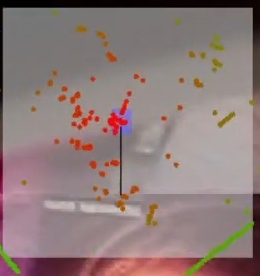
\includegraphics[width=0.8\textwidth]{./images/Pruebas/robot/MapaConRuidoSolar.png}
        \caption{Mapa con ruido por luz solar}
        \label{fig:MapaConRuidoLuzSolar}
    \end{figure}
    \clearpage
% subsection An\'alisis tercera  (end)